\section{Introduction}
\label{sec:intro}

Recent advances in large language models (LLMs)~\cite{chowdhery2022palm, brown2020language, scao2022bloom, bubeck2023sparks, openai2023gpt4, ChatGPT} have enabled significant new capabilities including natural dialogue, mathematical reasoning, and program synthesis. 
However, despite these advances, LLMs are still fundamentally limited by the information they can store in a fixed set of weights and the things they can compute using a static computation graph and limited context. 
Furthermore, as the world changes, LLMs require retraining to update their knowledge and reasoning capabilities. 

By empowering LLMs to use tools~\cite{schick2023toolformer}, we can grant access to vastly larger and changing knowledge bases and accomplish complex computational tasks.
By providing access to search technologies and databases, \cite{nakano2021webgpt, thoppilan2022lamda, shuster2022blenderbot} demonstrated that we can augment LLMs to address a significantly larger and more dynamic knowledge space. 
Similarly, by providing access to computational tools, \cite{thoppilan2022lamda, andor2019giving} demonstrated that LLMs can accomplish complex computational tasks. 
Consequently, leading LLM providers\cite{openai2023gpt4}, have started to integrate plugins to allow LLMs to invoke external tools through APIs.

This transition from a small set of hand-coded tools, to the ability to invoke a vast space of changing cloud APIs could transform LLMs into the primary interface to computing infrastructure and the web. 
Tasks ranging from booking an entire vacation to hosting a conference, could become as simple as talking to an LLM that has access to the flight, car rental, hotel, catering, and entertainment web APIs. 
However, much of the prior work~\cite{shen2023hugginggpt, liang2023taskmatrix} integrating tools into LLMs considered a small well documented set of APIs that can be easily injected into the prompt.

Supporting a web scale collection of potentially millions of changing APIs requires rethinking our approach to how we integrate tools.
It is not longer possible to describe the full set of APIs in a single context. 
Many of the APIs will have overlapping functionality with nuanced limitations and constraints. 
Simply evaluating LLMs in this new setting requires new benchmarks.



\begin{figure}[t]
    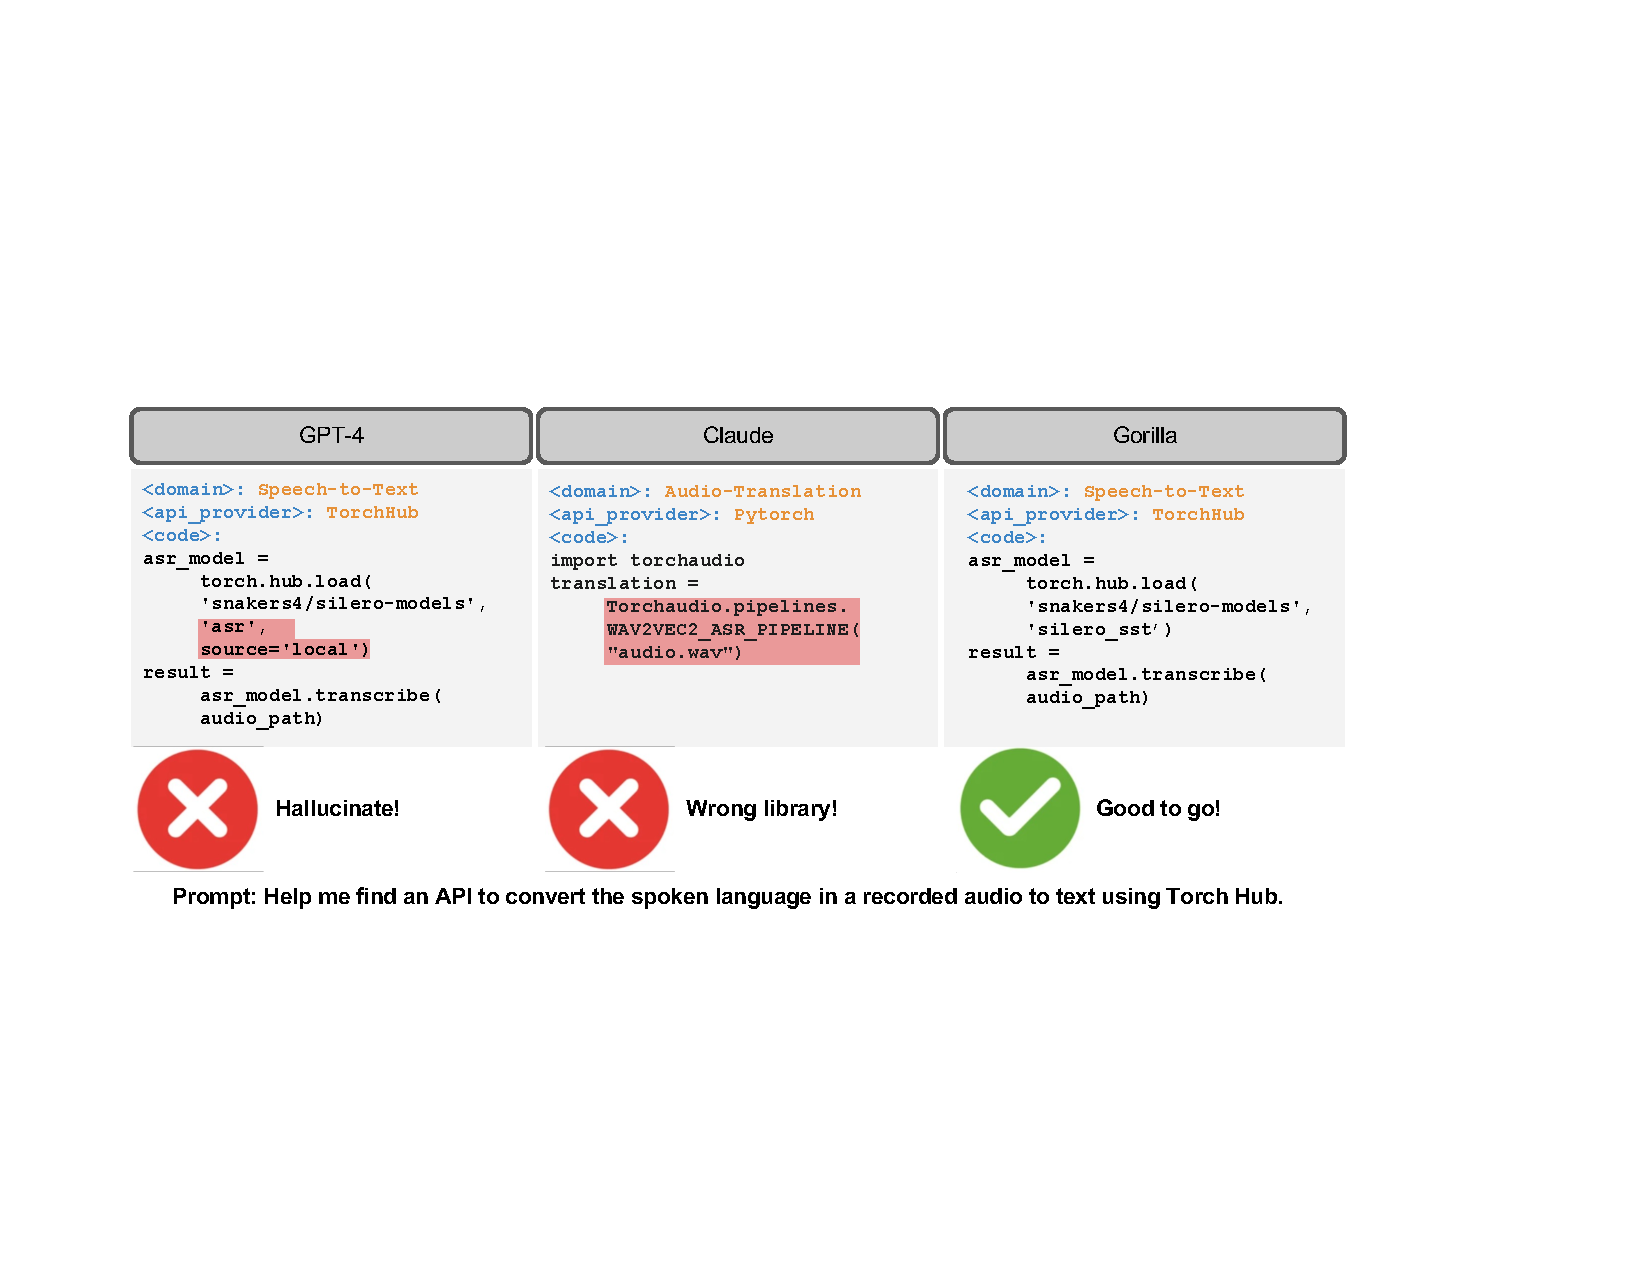
\includegraphics[width=\linewidth]{figures/code-examples.pdf}
\caption{\footnotesize \textbf{Examples of API calls}. Example API calls generated by GPT-4~\cite{openai2023gpt4}, Claude~\cite{Claude}, and \oursmethod{} for the given prompt. In this example, GPT-4 presents a model that doesn't exist, and Claude picks an incorrect library. In contrast, our \oursmethod{} model can identify the task correctly and suggest a fully-qualified API call.}
\label{fig:examplecode}
\end{figure}


In this paper, we explore the use of self-instruct fine-tuning and retrieval to enable LLMs to accurately select from a large, overlapping, and changing set tools expressed using their APIs and API documentation.
We construct, \oursdataset{}, a large corpus of APIs with complex and often overlapping functionality by scraping ML APIs (models) from public model hubs.  
We choose three major model hubs for dataset construction: TorchHub, TensorHub and HuggingFace. We exhaustively include every API call in TorchHub (94 API calls) and TensorHub (696 API calls); For HuggingFace, since the models come in a large number and lots of the models don't have a specification, we choose the most downloaded 20 models per task category (in a total of 925). We also generate 10 synthetic user question prompts per API using Self-Instruct~\cite{wang2022self}. Thus, each entry in the dataset becomes an instruction reference API pair. We adopt a common AST sub-tree matching technique to evaluate the functional correctness of the generated API. We first parse the generated code into an AST tree, then find a sub-tree whose root node is the API call that we care about (e.g., \texttt{torch.hub.load}) and use it to index our dataset. We check the functional correctness and hallucination problem for the LLMs, reporting the corresponding accuracy. 

We then finetune \oursmethod{}, a LLaMA-7B-based model with document retrieval using our dataset. We find that \oursmethod{} significantly outperforms GPT-4 in terms of API functionality accuracy as well as reducing hallucination errors. We show an example output in Fig.~\ref{fig:examplecode}.  Further, our retrieval-aware training of \gorilla{} enables the model to adapt to changes in the API documentation. Finally, we demonstrate Gorilla's ability to understand and reason about constraints.



\begin{figure}[t]
    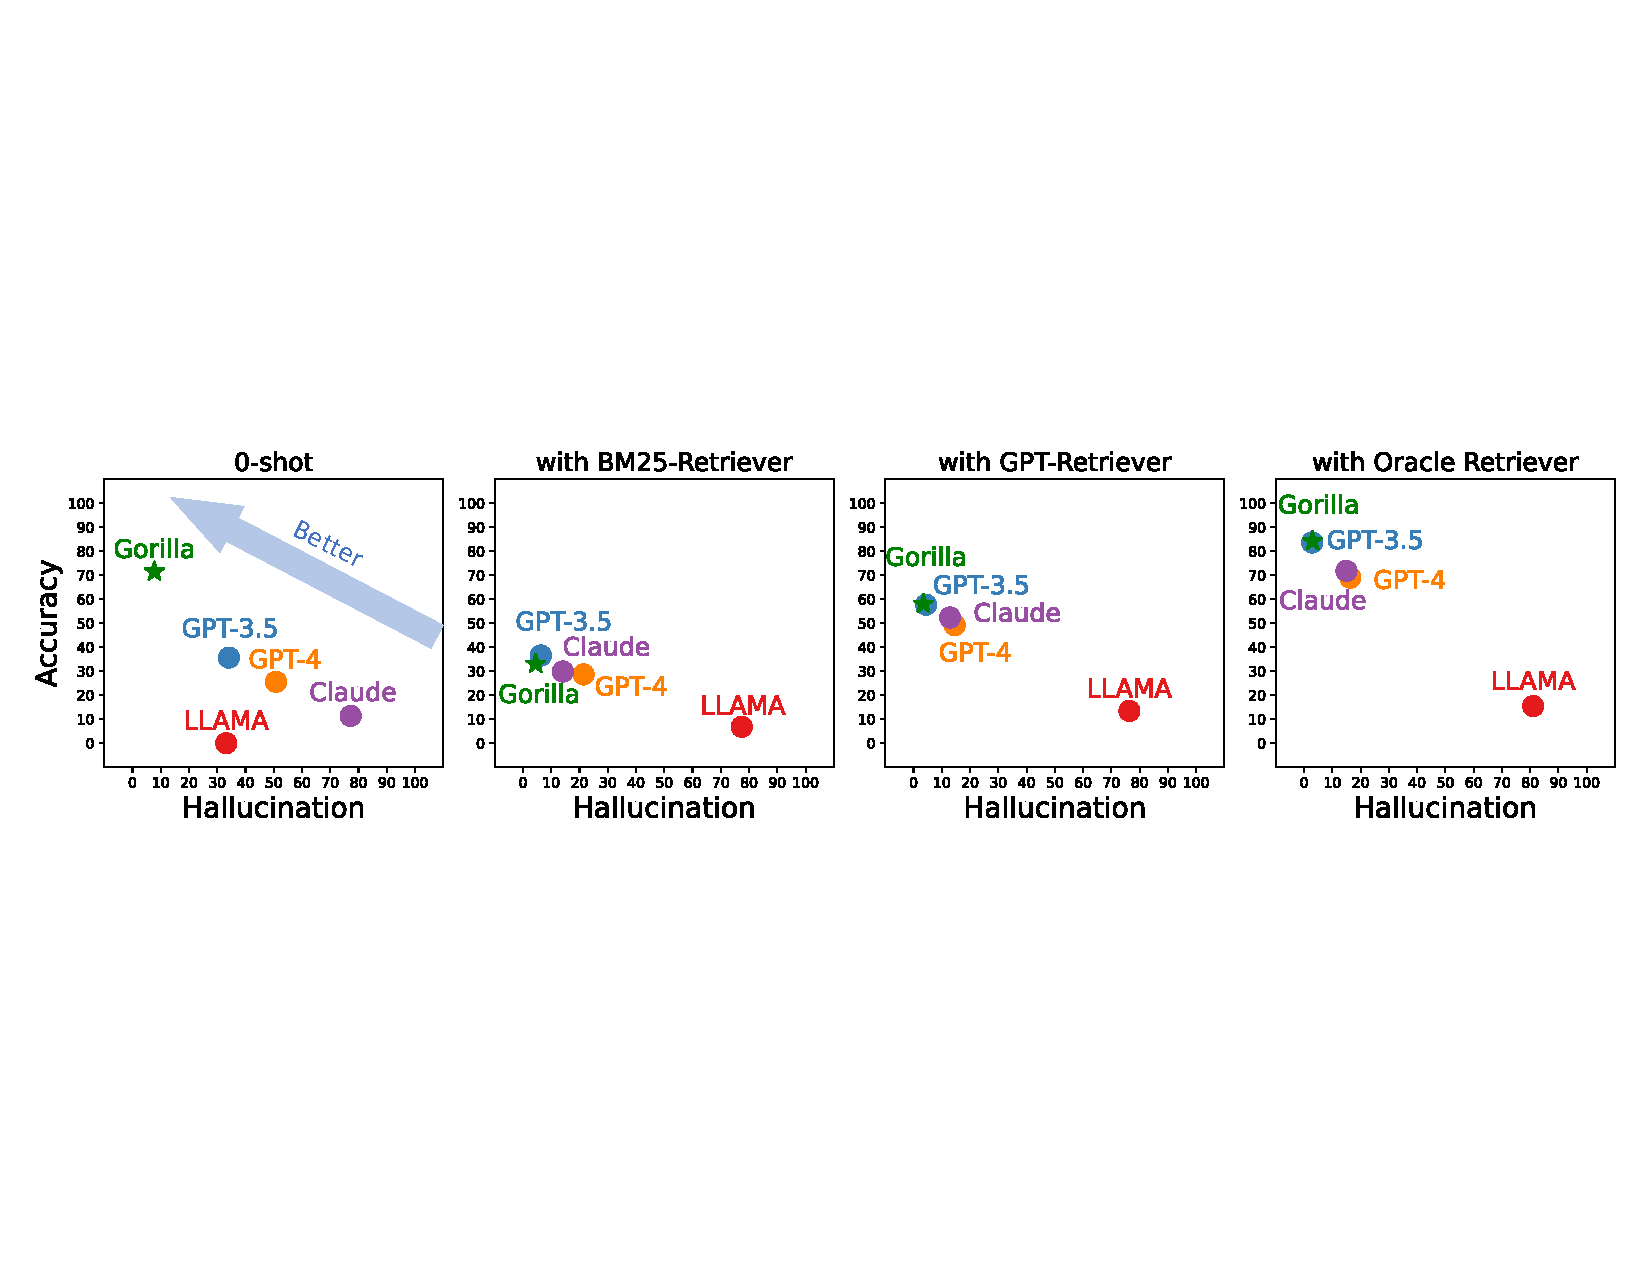
\includegraphics[width=\linewidth]{figures/average_grid.pdf}
\caption{\footnotesize \textbf{Accuracy (vs) hallucination} in four settings, that is,  \emph{zero-shot} (i.e., without any retriever), and \emph{with retrievers}. \texttt{BM25} and \texttt{GPT} are commonly used retrievers and the \texttt{oracle} retriever returns relevant documents at 100\%, indicating an upper bound. Higher in the graph (higher accuracy) and to the left is better (lower hallucination). Across the entire dataset, our model, \oursmethod{}, improves accuracy while reducing hallucination.}
\label{fig:acc-hallu}
\end{figure}


